\section{Quantum algorithms}

It's now to see some important quantum circuits that can be used in practice in order to obtain interesting results or behaviour inside a quantum computer. A lot of them will be not usefull per se, but are really important for the creation of larger and more powerful schemes.

\subsection{Quantum Fourier Transform}

The aim is to create an algorithm that bring the computational basis into the Fourier base, defined by the application of the Fourier transform on the vectors of the base itself. Therefore, we need first to recall the definition of discrete fourier transform which is given by.
\dfn{Discrete Fourier transform}
{
    Taken a vector $(x_1, x_2, \dots, x_N)\in \mathbb{C}^N$ it's Fourier transform is an application $\mathcal{U}: \mathbb{C}^N \to \mathbb{C}^N$ that actes in the following way
    \begin{align}
        &\mathcal{U}\vb{x} = \vb{y}, &y_k = \frac{1}{\sqrt{N}} \sum_{j=1}^N e^{i2\pi \frac{jk}{N}}x_j.
    \end{align} 
}
\noindent
We know that such an application posses a lot of properties, in particular we know how the following realtions are true
\begin{align}
    \label{eq:DiscrFourTrans}
    &\mathcal{U}^{-1} = \mathcal{U}^*, &\mathcal{U}^{-1} = \mathcal{U}^\dagger,
\end{align}
meanging that it's a particular unitary transformation, and so we imagine that a circuit can represent it.

We basically want to create an algorithm that allows us to take the computational basis and perform \eqref{eq:DiscrFourTrans} on it. In order to do that we will use a particular notation to describe the computational base of an $N$ qubit system, using the binary representation.
\dfn{Binary representation}
{
    Taken a system of $N$ qubit, where the computational base has the form $\{\ket{00\dots 0}, \ket{00\dots 1}, \dots\}$ we will write down the element s of the basis as $\{\ket{j}\}_{j=0}^{2^N-1}$ where the following relation is given
    \begin{align}
        &\ket{j} = \ket{j_1j_2\dots j_N}, &j = \sum_{i=1}^N j_i 2^{N-i}.
    \end{align}
    basically $j$ is the number described by the system state in binary base.
}
\noindent
Using this notation it's really easy to write down the Fourier transform of the base having that
\begin{equation}
    \label{eq:QFT}
    \mathcal{U}\ket{j} = \frac{1}{2^{N/2}} \sum_{k=0}^{2^N-1} e^{i2\pi \frac{jk}{2^N}} \ket{k},
\end{equation}
having that the base is brought into another more complicated one. In fact, we can see how the states transform accordingly to the FT if the transformation is applied to the base. For example take a general state $\ket{\psi}$ we can see how
\begin{align}
    &\ket{\psi} = \sum_j x_j \ket{j}, &\mathcal{U}\ket{\psi} = \frac{1}{2^{N/2}} \sum_k\sum_j x_j e^{i2\pi \frac{jk}{2^N}} \ket{k} = \sum_k y_k\ket{k},
\end{align}
basically the coefficients defining the state in vector representation gets Fourier transformed. Still, this form of the Fourier tranform leaves not too much room for the creation of an algorithm that allow us to perform it in practice, so we need first to work a little on it and see how the following result holds.
\thm{Quantum Fourier Tranform}
{
    The Fourier transformation of the states in the computational basis can be rewritten as a sum of tensor product given by the following form using the binary representation for the base
    \begin{equation}
        \mathcal{U}\ket{j} = \frac{1}{2^{N/2}}\bigotimes_{l=1}^N\left[ \ket{0}_l + e^{i2\pi \mathbb{0}_j(N-l)}\ket{1}_l \right].
    \end{equation}
    Where the notation $\mathbb{0}_j(l)$ is defined as the following decimal number
    \begin{align}
        \label{eq:decimalForm}
        &\mathbb{0}_j(l) = \sum_{i=l+1}^N j_i2^{l - i}.
    \end{align}
}
\pf{Proof}
{
    We can start to work around the expression of \eqref{eq:QFT} by seing how we can rewrite $k/2^{N}$ in a more usefull form as
    \begin{equation}
        \frac{k}{2^N} = \sum_{l=1}^N k_l 2^{-l}.
    \end{equation}
    We can then substitute it and see how, recalling that $\ket{k} = \ket{k_1}\otimes\ket{k_2}\dots\otimes\ket{k_N}$, the following is true
    \begin{equation}
        \mathcal{U}\ket{j} = \frac{1}{2^{N/2}} \sum_{k=0}^{2^N-1} e^{i2\pi j\sum_{l=1}^N k_l 2^{-l}} \ket{k} = \frac{1}{2^{N/2}}\sum_{k=0}^{2^N - 1}\bigotimes_{l=1}^N e^{i2\pi jk_l 2^{-l}}\ket{k_l}.
    \end{equation}
    Now, the order of the operation can be inverted by taking some care anbd see how the expression become
    \begin{equation}
        \mathcal{U}\ket{j} = \frac{1}{2^{N/2}}\bigotimes_{l=1}^N \sum_{k_l = 0, 1}e^{i2\pi jk_l 2^{-l}}\ket{k_l} = \frac{1}{2^{N/2}}\bigotimes_{l=1}^N\left[ \ket{0}_l + e^{i2\pi j2^{-l}}\ket{1}_l \right].
    \end{equation}
    Now, we can see how the exponent can be simplified. In fact, if you use the definition of $j$ we can see how
    \begin{equation}
        j2^{-l} = \sum_i j_i 2^{N - i - l} = \sum_{i \le N-l} j_i 2^{N - i - l} + \sum_{i = N-l+1}^N j_i 2^{N - i - l} = \text{integer} + \mathbb{0}_j(N-l).
    \end{equation}
    Obviously the integer part gives no contribution to the phase since multiply $2\pi$ at the exponent, so only the $\mathbb{0}_j(N-l)$ can be written obtaining the final result.
}

\begin{figure}[t]
    \centering
    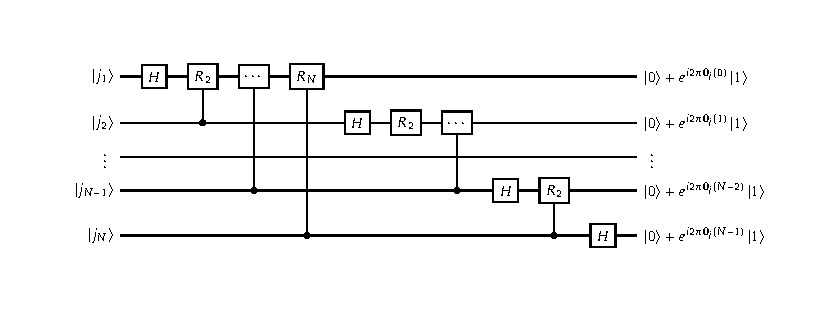
\includegraphics[width=0.9\textwidth]{Immagini/QFT.pdf}
    \caption
    {
        Circuits able to perform the quantum fourier tranform of the computational basis. It's important to notice how this algorithm is in reality not totally complete since the phases of the final states are inverted, so a series of swap gates needs to be inserted at the end to get the right form.
    }
    \label{fig:QFT}
\end{figure}
Now, this form of the QFT is much more usefull on an algorithmic point of view since it's now easy per us to see the operations that needs to be done on the single qubits. In particular, to reproduce the result we will need two types of gates that are also easy to understand that are
\begin{align}
    &H = \frac{1}{\sqrt{2}}\begin{pmatrix}
        1 & 1\\
        1 & -1
    \end{pmatrix},
    &R_k = \begin{pmatrix}
        1 & 0\\
        1 & e^{1\frac{2\pi}{2^k}}
    \end{pmatrix},
\end{align}
basically the Hadamart and phase gates. The final form of the circuit is described in \figref{fig:QFT}, where is possible to see how we can evaluate the QFT by the cimple use of controlled phase gates and swaps ones at teh end of the proces. This particular circuit is interesting since shows how quantum computers are able to perform fuorier transforms easily respect to classical algorithm. In fact, the number of gates required to perform such an operation scales as $\mathcal{O}(n^2)$ while the number of logic gates needed to perform the computation of a fast fourier transform inside a classical computer scales as $\mathcal{O}(n2^n)$. Quantum algorithm beats the classical one by an exponential factor. Nevertheless, the quantum algorithm has the big problem that the information are present in the phase of the states, and we are not able to evaluate them, basically meaning that the algorithm alone is useless. Still, we will see that QFT will still be used inside larger algorithm giving a lot of benefits.

\subsection{Phase evaluation}

The evaluation of phases inside quantum systems is always a troublesome problem, to the point that most of the time is thought as an impossible task. Nevertheless, is possible to see how the QFT algorithm is able to give us the possibility of experimentally evaluate a certain type of phase inside the system.

Let's imagine having a unitary operator $\mathcal{U}$ and wanting to evaluate the eigenvalues $\lambda_n$. We know from linear algebra that $\mathcal{U}\mathcal{U}^\dagger = \mathbb{1}$, so that from linear algebra we have the following information on the eigenvalues
\begin{align}
    &\lambda_n\lambda_n^* = \abs{\lambda_n}^2 = 1.
\end{align}
This relation tells us that the eigenvalues of such opeartors needs to be some kind of complex phases writable as
\begin{align}
    &\lambda_n = e^{2\pi i \phi_n}, &\phi_n \in [0, 1[.
\end{align}
Normally we would think that evaluating $\phi_n$ would be impossible since phases cannot be observed axperimentally. Still, we will show how using the eigenstate of the phases $\ket{u_n}$ and a simple operator $\mathcal{U}^{2^j}$ defined as follows
\begin{equation}
    \mathcal{U}^{2^j}: \ket{u_n} \longmapsto e^{2\pi i \phi_n 2^j} \ket{u_n},
\end{equation}
we are able to approximate its value with a wanted precision. In particular, we are aiming to approximate $\phi_n$ using a decimal form like the one in \eqref{eq:decimalForm}, so that we want to find $(b_n^1, b_n^2, \dots, b_n^t)$ so that 
\begin{equation}
    b_n = \frac{b_n^1}{2} + \frac{b_n^2}{4} + \dots + \frac{b_n^t}{2^t},
\end{equation}
is the decimal number $b < \phi_n$ closer to it as possible. Therefore, we are going to demonstrate that the algorithm showed in \figref{fig:Phase} is able to do exactly that, find out the values of $b_n^i$ approximating the phase up to a wanted accuracy.

\begin{figure}[t]
    \centering
    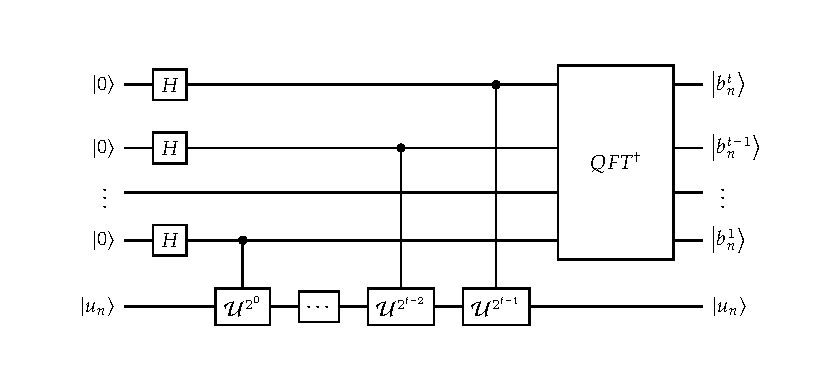
\includegraphics[width=0.8\textwidth]{Immagini/Phase.pdf}
    \caption
    {
        Quantum circuit for the approximation of the eigenvalues of a unitary operator up to a wanted accuracy based on the number of qubit used for the decimal approximation of the phase itself.
    }
    \label{fig:Phase}
\end{figure}

\thm{Phase evaluation}
{
    Taken a unitary operator $\mathcal{U}$ with eigenvalues defined by the phases $\phi_n$, the circuit \figref{fig:Phase} is able to give as output its decimal approximation $b_n$ with a wanted accuracy $\alpha > 0$, and precision $\epsilon > 0$ if the number of qubit used for the operation is
    \begin{equation}
        \label{eq:PhaseEvaluation}
        t > \alpha + \ln\left( 2 + \frac{1}{2\epsilon} \right).
    \end{equation}
}
\pf{Proof}
{
    First we need to look at what the circuit does effectivelly to the states, and it's easy to see that by looking at the case where $t = 1$ and see how the first part of the circuit works as follows
    \begin{equation}
        \left(C\mathcal{U}^{2^0}\right)\left(H\otimes\mathbb{1}\right)\ket{0}\otimes\ket{u_n} = C\mathcal{U}^{2^0}\left( \frac{\ket{0} + \ket{1}}{\sqrt{2}} \right)\otimes\ket{u_n} = \left( \frac{\ket{0} + e^{2\pi i\phi_n}\ket{1}}{\sqrt{2}} \right)\otimes\ket{u_n}.
    \end{equation}
    Which can be easily generalized to all the applications on the genearal $t$-dimensional circuit having a final form of the state given by
    \begin{equation}
        \ket{\psi_f} = \left[\bigotimes_{j = 0}^{t-1}\left( \frac{\ket{0} + e^{2\pi i\phi_n2^j}\ket{1}}{\sqrt{2}} \right)\right]\otimes\ket{u_n}
    \end{equation}
    Now, we know how every real number can be written as a converging series of rational numbers such as \eqref{eq:decimalForm} so that we are going to work with
    \begin{equation}
        \label{eq:rationalApproxPhase}
        \phi_n = \frac{\phi_n^1}{2} + \frac{\phi_n^2}{4} + \dots = \sum_{i=1}^\infty \frac{\phi_i}{2^i} \approx \sum_{i=1}^t \frac{\phi_i}{2^i}.
    \end{equation} 
    Meaning that can be approximated using the decimal representation described before, having that the phases can be rewritten using the following form
    \begin{equation}
        \exp\left( 2\pi i \phi_n 2^j \right) = \exp\left( 2\pi i\left\{ \left[ \phi_n^1 2^{j-1} + \dots \right] + \left[ \phi_n^{j+1}2^{-1} + \dots \right] \right\} \right) = \exp\left( 2\pi i \mathbb{0}_\phi(j) \right),
    \end{equation}
    where the first part was an integer giving no contribution. In this way one can understand that in the first part of the $\ket{\psi_f}$ state we end up having the QFT of the initial states, allowing us to write it in binary representation as
    \begin{equation}
        \ket{\psi_f} \approx \left( \frac{1}{2^{t/2}}\sum_{k=0}^{2^t-1}e^{2\pi i\phi_nk}\ket{k} \right)\otimes\ket{u_n}.
    \end{equation}
    In this way we can go and apply the inverse of the QFT and using the binary representation of the base to see what happens exactly in the transformation
    \begin{equation}
        QFT^\dagger \ket{\psi_f} = \frac{1}{2^t}\sum_{k=0}^{2^t-1} e^{2\pi i\phi_nk}\sum_{l=0}^{2^t-1} e^{-2\pi ikl/2^t}\ket{l} = \sum_l\left( \sum_{k=0}^{2^t-1}\frac{1}{2^t}e^{2\pi i (\phi_n - l/2^t)k} \right)\ket{l} = \sum_l c_l\ket{l}.
    \end{equation}
    The state becomes a superposition of states in the binary computational base of the $t$ qubits, and we know also the form of the coefficients. In fact, we can easily see how $c_l$ are composed by a geometric series giving rise to the following result
    \begin{equation}
        \label{eq:CoeffPhase}
        c_l = \frac{1}{2^t} \sum_{k=0}^{2^t-1} \left( e^{2\pi i (\phi_n - l/2^t)} \right)^k = \frac{1}{2^t}\frac{1 - e^{2\pi i (\phi_n - l/2^t)2^t}}{1 - e^{2\pi i (\phi_n - l/2^t)}}.  
    \end{equation}
    It's interesting to see how this result was obtained by truncating the real form of $\phi_n$ to a certain decimal order, but the procedure is general and works also in the case where the total series is retained. 
    
    Therefore, in \eqref{eq:CoeffPhase} the value of $\phi_n$ can be a rational or irrational number, and we can see what happens to $c_l$ in the two cases. In the case $\phi_n$ is rational we have that the approximation \eqref{eq:rationalApproxPhase} is exact, and we can write how
    \begin{equation}
        (\phi_n - l/2^t)2^t = \sum_{i=1}^t \phi_n^i 2^{t-i} -l = int.
    \end{equation}
    This means that the phase on the numerator of $c_l$ is a multiple of $2\pi$ and therefore $c_l = 0$ for every value of $l$ exept for $l=\phi_n 2^t$, where
    \begin{equation}
        c_{\phi_n2^t} = \frac{1}{2^t} \sum_{k=0}^{2^t-1} \left( e^{2\pi i (\phi_n - \phi_n)} \right)^k = \frac{2^t}{2^t} = 1.
    \end{equation}
    This means that $c_l = \delta_{l\phi_n2^t}$ which basically becomes a condition on the values of the single qubit that will take the following forms
    \begin{equation}
        \sum_{l=0}^{2^t-1} \delta_{l\phi_n2^t}\ket{l} = \ket{\phi_n2^t} = \ket{\phi_n^1}\otimes\ket{\phi_n^2}\otimes\dots\otimes\ket{\phi_n^t}, 
    \end{equation}
    where the binary representation was used to write down the single qubits. Now, we can simply evaluate all the $t$ qubits and have our approximation of the phase $\phi_n$ that is exact in this case, having that $b_n = \phi_n$.

    In the case $\phi_n$ is irrational, the truncation in the series generate an error having also that $(\phi_n - l/2^t)2^t$ is not an integer anymore and $c_l$ can be different from $0$ for other $l$ values. In this case we are going to approximate the value of $\phi_n$ using the values of $b_n$ that we obtain from the evaluation, and we want to know the error we are generating from such an approximation along with the accuracy of the result. Therefore, we select an error value $\omega$ and compute the probability of performing the measure 
    \begin{equation}
        \tilde{P} = P(\overline{l} \in [-\omega-1, \omega+1]),
    \end{equation}
    where $\overline{l} = l - \phi_n$ so that $\overline{l} = 0$ correspond to the real $\phi_n$. This evaluation can be performed using as $\omega$ the value $2^{t - \alpha} - 1$, where $\alpha$ is called accuracy, obtaining the result of
    \begin{equation}
        1 - \tilde{P} \le \frac{1}{2(2^{t-\alpha} - 2)}.
    \end{equation}
    Which identify the probability of not obtaining the wanted result, that we are going to set below a certain precision $\epsilon$ having $1 - \tilde{P}<\epsilon$ so that the following relations is found
    \begin{equation}
        t > \alpha + \ln\left( 2 + \frac{1}{2\epsilon} \right).
    \end{equation}
}
\noindent
Therefore, this algorithm is able to give us a really greate approximation for the phase that increase in accuracy as we scale up the number of qubit used in order to perform the operation. Also, it's possible to see how we from the inequality we can actually controll also the accuracy and precision of the prediction by setting them prior and then choose $t$ in order to satisfy \eqref{eq:PhaseEvaluation}.